\documentclass[border=5pt 5pt 5pt 5pt]{standalone}

\usepackage{tikz}

\begin{document}

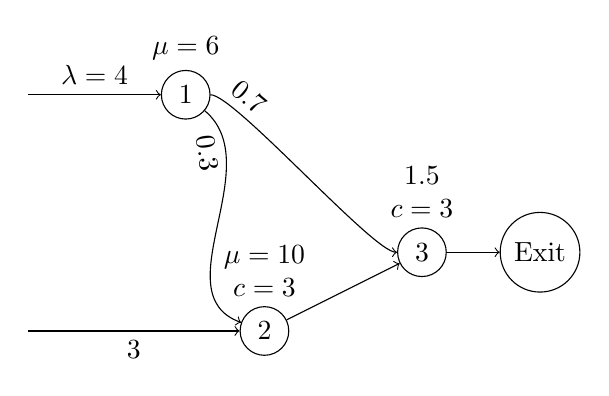
\begin{tikzpicture}
    % Service nodes
    \node at (2, 3) [circle,draw,label={[align=center]$\mu=6$}] (1) {1};
    \node at (3, 0) [circle,draw,label={[align=center]$\mu=10$\\$c=3$}] (2) {2};
    \node at (5, 1) [circle,draw,label={[align=center]$1.5$\\$c=3$}] (3) {3};
    \node at (6.5, 1) [circle,draw] (exit) {Exit};

    % Arrival arrows
    \draw[->] (0, 3) to node[midway,above] {$\lambda=4$} (1) ;
    \draw[->] (0, 0) to node[midway,below] {$3$} (2);

    % Other arrows
    \draw[->] (1) to[looseness=1,out=320,in=160] node[pos=0.2,below,sloped]
    {0.3} (2);
    \draw[->] (1) to[looseness=0.25,out=0,in=180] node[pos=0.2,above,sloped]
    {0.7} (3);
    \draw[->] (2) to (3);
    \draw[->] (3) to (exit);
\end{tikzpicture}

\end{document}
